\lecture\begin{rem}
	Wegen \ref{6.12} ist die Definition von $d_g$ unabhängig von der Koordinatenwahl in $M$.
\end{rem}

\begin{rem}
	Direkt aus der Definition sieht man:
	\begin{itemize}
		\item $ d(p,p) = 0, d(p,q) \geq 0 $
		\item $ d(p,q) = d(q,p) $ ($L(\gamma)$ ist unabhängig von der Umlaufrichtung)
		\item $ d(p,q) \leq d(p,\tilde{q}) + d(\tilde{q},q) $
	\end{itemize}
\end{rem}

\begin{thm}
	$ (M,d_g) $ ist ein metrischer Raum.
\end{thm}

\begin{lem}
	Sei $ p \in M,$ $(M,g) $ eine Riemannsche Mannigfaltigkeit. Dann ist $ f:= d_g(\cdot,p) $ stetig.
\end{lem}

\begin{cor}
	Die Topologie auf $ (M,g) $, die von $d_g$ induziert wird, ist die selbe wie die Topologie auf $M$ als Mannigfaltigkeit.
\end{cor}

\begin{lem}
	Sind $ (M,g_M), (N,g_N) $ zusammenhängende Riemannsche Mannigfaltigkeiten, $ f:M \to N $ eine Isometrie, so gilt
	\[ d_{g_N}(f(p),f(q)) = d_{g_M}(p,q) \quad \foralll p,q \in M. \]
\end{lem}

\begin{rem*}
	Lokale Isometrien können in der Tat Länge verkürzen.\\
	\begin{minipage}{\linewidth}
		\begin{wrapfigure}{r}{4cm}
			%			\centering
			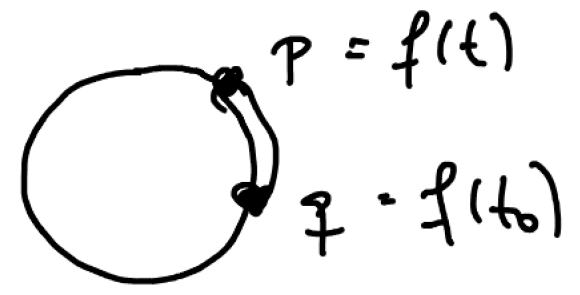
\includegraphics[width=4cm]{6_18 rem.png}
		\end{wrapfigure}
		$ f: \R \to \R^2$\\
		$f(t) = (\cos(t),\sin(t)) $ ($ \im(f) = \Sbb^1 $)\\
		$ d_{\Sbb^1}(p,q) = $ Bogenlänge = $ |t-t_0| \mod 2\pi $\\
		$ d_\R(t,t_0) = |t-t_0| \geq |t-t_0| \mod 2\pi $
	\end{minipage}
\end{rem*}

\begin{cor*}
	Eine zusammenhängende Riemannsche Mannigfaltigkeit $M$ ist genau dann \emph{vollständig} (als topologischer Raum) wenn $(M,d_g)$ vollständig ist (als metrischer Raum).\\
	Und: Es ist sinnvoll, eine Teilmenge $ A \subset M $ beschränkt zu nennen, falls $ \existss C \geq 0 $, sodass $ d_g(q,p) \leq C \ \foralll q,p \in A. $
\end{cor*}

\begin{exmp*}[nicht vollständig:]
	$ \Sbb^2 \setminus \{p\} $\\
	$ d(q_1,q_2) = $ Bogenlänge der Verbindung auf dem (kürzeren) Großkreis
	\image{6_18 exmp}{3cm}
\end{exmp*}

\begin{rem*}
	"Geodäte" =  eine kürzeste Verbindung zwischen zwei Punkten.\\
	Muss nicht existieren (siehe oben)
\end{rem*}

\begin{rem}
	$ \hat{g}: TM \to T^*M, \hat{g}(v)(w) := g_p(v,w) \ \foralll v,w \in T_pM $\\
	$ Y \mapsto \hat{g}(X)(Y) $ ist $C^\infty$-linear, $X,Y \in \Xfrak(M)$\\
	\ref{4.7} $\implies \hat{g}(X)$ ist ein glattes Vektorfeld \checkmark \\
	$\hat{g}$ ist ein Isomorphismus:\\
	injektiv wegen $\hat{g}(v) = 0 \implies 0 = \langle v,v\rangle_g \implies 0$\\
	$\implies$ (Dimensionsformel) $\hat{g}$ surjektiv.
\end{rem}

\begin{defn*}[Gradient]
	Sei $f: M \to \R$ glatt auf $(M,g)$. Der \emph{Gradient} von $f$ ist
	\[ \grad f = \hat{g}^{-1}(df) \in \Xfrak(M) \]
\end{defn*}

\begin{rem*}
	\begin{enumerate}[label={\roman*})]
		\item Für $ M = \R^n, g = \bar{g}, $ ist $ \grad f = (\del{1}f \dots \del{n}f) $
		\item Es gilt $ \foralll X \in \Xfrak(M): $\\
			$ \langle \grad f, X \rangle_g = \hat{g} (\grad f)(X) = df(X) = X \cdot f $
		\item $\grad f$ zeigt in Richtung des stärksten Anstiegs und steht orthogonal auf den Höhenlinien.
	\end{enumerate}
\end{rem*}

\begin{exmp*}
	$\bar{g}$ in Polarkoordinaten: $ \begin{pmatrix}
		1&0\\0&r^2
	\end{pmatrix},\ \bar{g}^{-1} = \begin{pmatrix}
	1&0\\0&\frac{1}{r^2}
	\end{pmatrix} $\\
	$ \implies \grad f  = \del{r}f \cdot \del{r} + \frac{1}{r^2} \del{\theta}f \cdot \del{\theta} $
\end{exmp*}